Two  banana  plugs  $X_{6A}$  and  $X_{6B}$  provide  the  connection  to  the
output  voltage,  while  reverse  voltage protection  is  achieved  via  diode
$V_4$.   (Figure \label{fig:circuit:output}).   An external  reference voltage
of  \SI{1.5}{\volt}  is  used to  ensure  that  the  ADCs  and DACs  can  make
accurate  measurements and  can  be used  over their  full  range (see  figure
\ref{fig:circuit:vref}).

\begin{minipage}{.50\textwidth}
    \center
    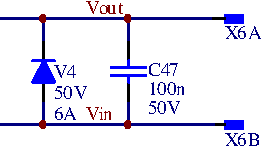
\includegraphics[width=.9\textwidth]{images/circuit/output-connectors.pdf}
    \captionof{figure}{Reverse voltage protection at output}
    \label{fig:circuit:output}
\end{minipage}
\begin{minipage}{.50\textwidth}
    \center
    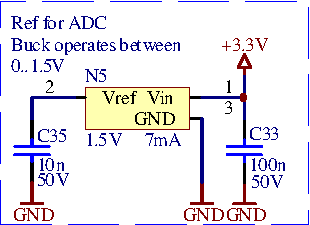
\includegraphics[width=.8\textwidth]{images/circuit/vref.pdf}
    \captionof{figure}{%
        \SI{1.5}{\volt} reference voltage for full-range operation of DACs
        and DACs
    }
    \label{fig:circuit:vref}
\end{minipage}

